\renewcommand{\thefigure}{A\arabic{figure}}
\setcounter{figure}{0}
\section*{Anexo}
%//==============================--@--==============================//%
\def\varQR{(2*pi*1.8)^2}
\def\varQRR{(2*pi*0.45)^2}
\def\fnum{-1/(2*2*pi*1.8)+sqrt(1/(4*(2*pi*1.8)^2)+1)}
\def\fndois{1/(2*2*pi*1.8)+sqrt(1/(4*(2*pi*1.8)^2)+1)}
\def\fntres{-1/(2*2*pi*0.45)+sqrt(1/(4*(2*pi*0.45)^2)+1)}
\def\fnquatro{1/(2*2*pi*0.45)+sqrt(1/(4*(2*pi*0.45)^2)+1)}

\tikzset{every node/.style={fill=white}}
\begin{figure}[!h]  
    \centering
    \resizebox{0.75\textwidth}{!}{%
        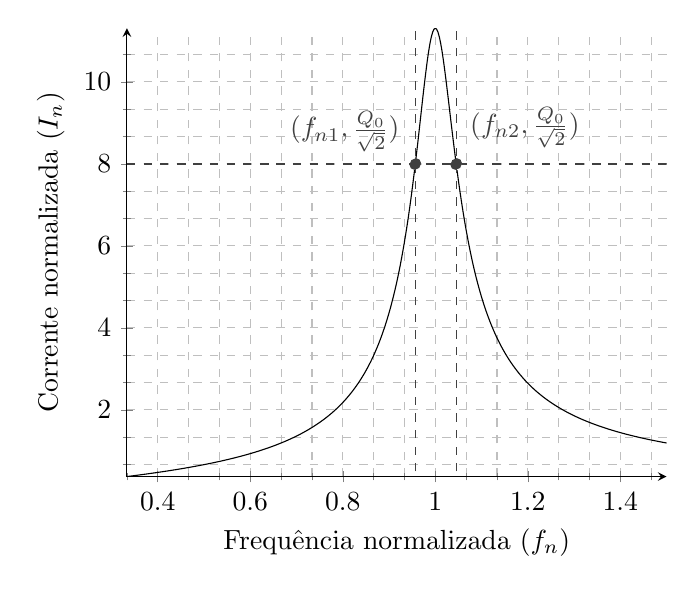
\begin{tikzpicture}
            \begin{axis}[
                axis lines = left,
                xlabel = {Frequência normalizada ($f_n$)},
                ylabel = {Corrente normalizada ($I_n$)},
                grid style=dashed,
                grid=both,
                minor tick num=2
            ]

            \addplot [
                domain=(1/3):(3/2), 
                samples=400, 
                color=black,
            ]
            { 1/sqrt( 1/(\varQR) + (x-1/x)^2 )};
            
            \addplot[
                domain=(1/3):(3/2), 
                samples=300, 
                color=darkgray,
                dashed
            ]
            {2*pi*1.8/sqrt(2)};
            
            \addplot [only marks,mark=*,dashed,color=darkgray] coordinates { (\fnum,2*pi*1.8/sqrt(2)};
            \node[label={160:{\color{darkgray} $(f_{n1},\frac{Q_0}{\sqrt{2}})$}},inner sep=2pt] at (0.956757,7.997189) {};
            
            \addplot [only marks,mark=*,dashed,color=darkgray] coordinates { (\fndois,2*pi*1.8/sqrt(2)};
            \node[label={55:{\color{darkgray} $(f_{n2},\frac{Q_0}{\sqrt{2}})$}},inner sep=2pt] at (1.045186,7.997189) {};
            
            \addplot +[mark=none,color=darkgray,dashed] coordinates {(\fnum, 0.5) (\fnum, 2*pi*1.8)};
            
            \addplot +[mark=none,color=darkgray,dashed] coordinates {(\fndois, 0.5) (\fndois, 2*pi*1.8)};
            
            %\addlegendentry{}
            \end{axis}
        \end{tikzpicture}
    }%
\caption{Curvas de corrente normalizada para $R=R_S=100\ \Omega$.} \label{fig:curvas_ressonancia100_anexo} 
\end{figure}

\begin{figure}[!h] 
    \centering
    \resizebox{0.75\textwidth}{!}{%
        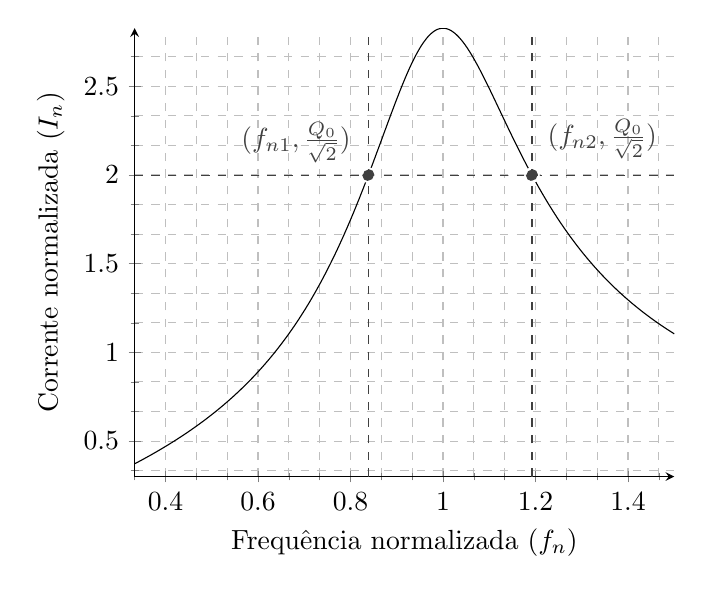
\begin{tikzpicture}
            \begin{axis}[
                axis lines = left,
                xlabel = {Frequência normalizada ($f_n$)},
                ylabel = {Corrente normalizada ($I_n$)},
                grid style=dashed,
                grid=both,
                minor tick num=2
            ]

            \addplot [
                domain=(1/3):(3/2), 
                samples=400, 
                color=black,
            ]
            { 1/sqrt( 1/(\varQRR) + (x-1/x)^2 )};
            
            \addplot[
                domain=(1/3):(3/2), 
                samples=300, 
                color=darkgray,
                dashed
            ]
            {2*pi*0.45/sqrt(2)};
            
            \addplot [only marks,mark=*,dashed,color=darkgray] coordinates { (\fntres,2*pi*0.45/sqrt(2)};
            \node[label={160:{\color{darkgray} $(f_{n1},\frac{Q_0}{\sqrt{2}})$}},circle,inner sep=2pt] at (0.838677,1.999297) {};

            \addplot [only marks,mark=*,dashed,color=darkgray] coordinates { (\fnquatro,2*pi*0.45/sqrt(2)};
            \node[label={45:{\color{darkgray} $(f_{n2},\frac{Q_0}{\sqrt{2}})$}},circle,inner sep=2pt] at (1.192354,1.999297) {};
            
            \addplot +[mark=none,color=darkgray,dashed] coordinates {(\fntres, 0.3) (\fntres, 2*pi*0.45)};
            
            \addplot +[mark=none,color=darkgray,dashed] coordinates {(\fnquatro, 0.3) (\fnquatro, 2*pi*0.45)};
            %\addlegendentry{}
            \end{axis}
        \end{tikzpicture}
    }%

\caption{Curvas de corrente normalizada para $R=R_S=400\ \Omega$.} \label{fig:curvas_ressonancia400_anexo} 
\end{figure}
%//==============================--@--==============================//%